\section{Runtime View}
In this section the runtime view of the system will be analyzed. It shows in detail how the system works in every use case, 
presenting the interaction between the internal components, discussed in the section 2.2, talking about Component View.

\subsection{Registration}
The diagram shows the workflow of the application during the registration. The behavior of 
the system is the same for normal user and authority, because authority first registers as a normal user, then updates the profile. The main 
component is the \textbf{UserModule} that contains the logic to check correctness of data for registration. The module communicates with RDBMS
to check if creation of user account is possible. In positive case the Client Application can choose the way to confirm account creation (whether
mobile phone number or email), and only after confirmation of data, the module inserts new user data into the RDBMS. In case of failure, an error 
message is sent back to the Client Application to communicate it. 

\begin{figure}[H]
  \centering
  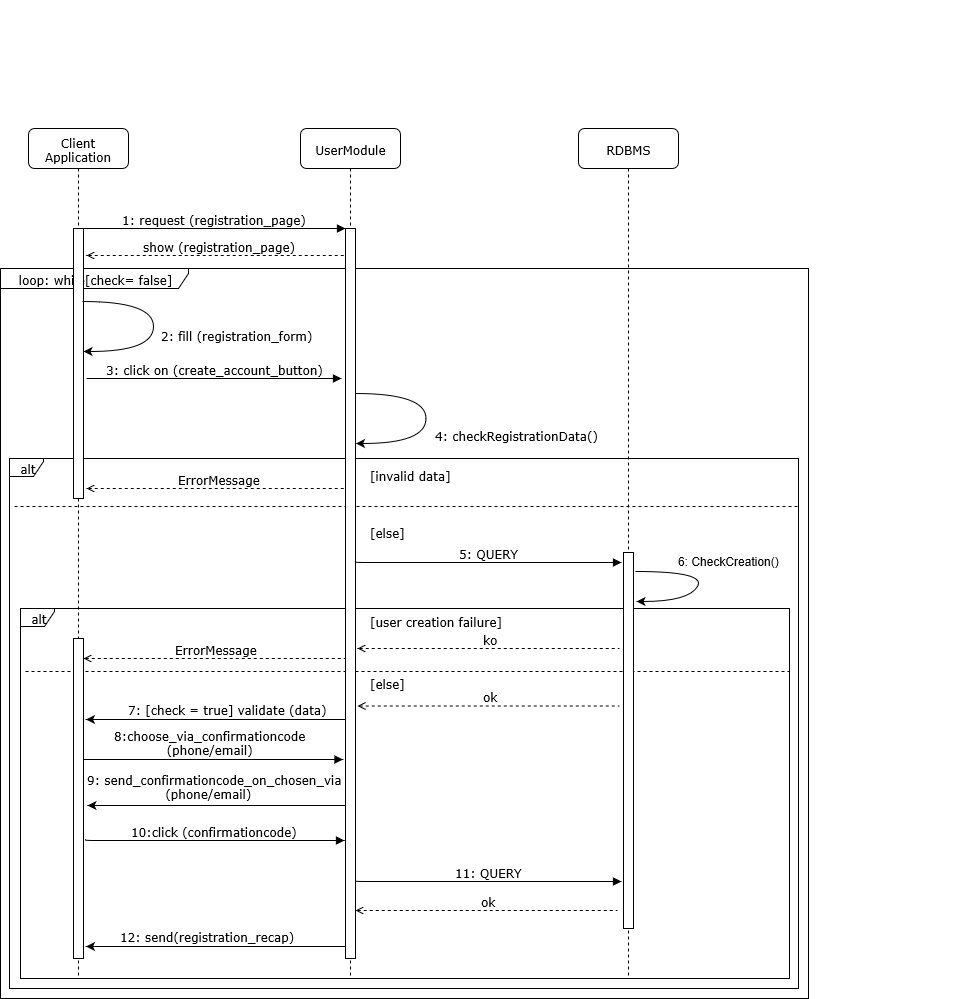
\includegraphics[width=\textwidth]{DD_Images/RunTimeView/1.jpg}
  \caption{\textit{Sequence diagram 1 - Registration}}
\end{figure}

\subsection{Submit of report}
The diagram shows the workflow of the application during the sending of a report from Client Application. The main 
component is the \textbf{ReportModule} that contains the logic to check correctness of data regarding report, and has the task to collect all
data regarding the provided report. The module communicates with ReportValidationModule for further confirmation of data. In this workflow 
the syntactic correctness of the received report is checked.  

\begin{figure}[H]
  \centering
  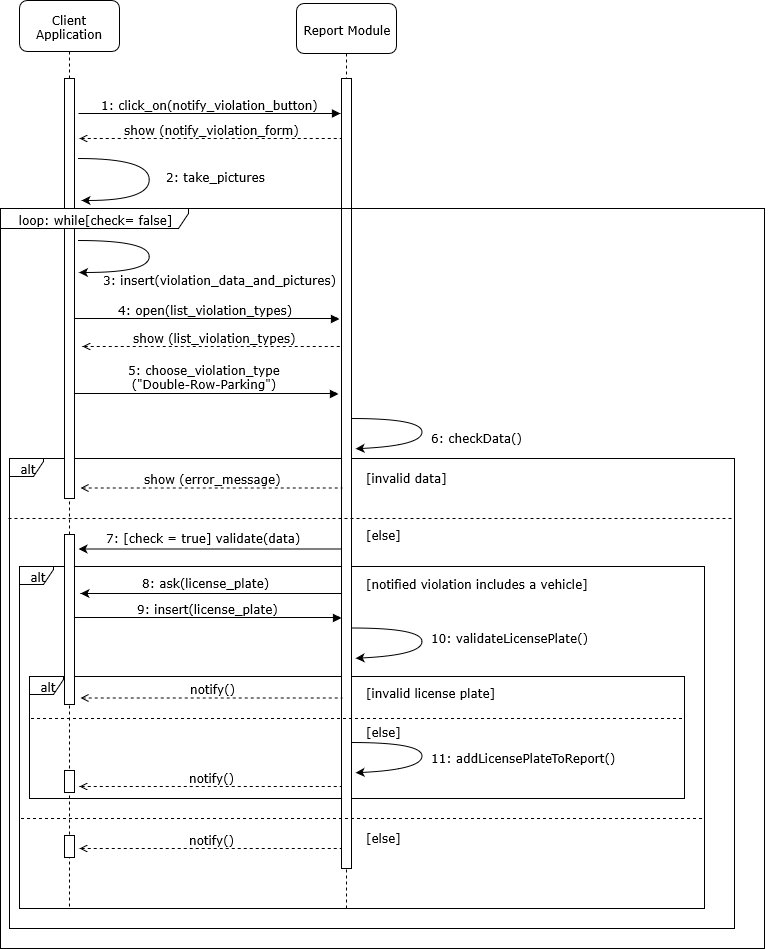
\includegraphics[width=\textwidth]{DD_Images/RunTimeView/2.jpg}
  \caption{\textit{Sequence diagram 2 - Submit of report}}
\end{figure}

\subsection{Validation of report}
The diagram shows the workflow of the application during the validation of a report. The system shows the interaction between two core 
modules, the \textbf{ReportModule} and the \textbf{ReportValidationModule}. The report, once accepted by the ReportModule, is submitted to
the ReportValidationModule, that contains all the logic to validate the report and communicate with the Client Application through the Notification
Push, to send all Client Applications the poll to answer to validate the report. Once the report has been validated the ReportValidationModule
registers the violation, inserting new data into the RDBMS. In case of absence of confirmation by the Client Applications to the poll, if the 
report is proved to be inconsistent and wrong, as rejected by a sufficient number of other clients, the ReportValidationModule updates RDBMS data 
assigning a penalty to the client who submitted the report.

\begin{figure}[H]
  \centering
  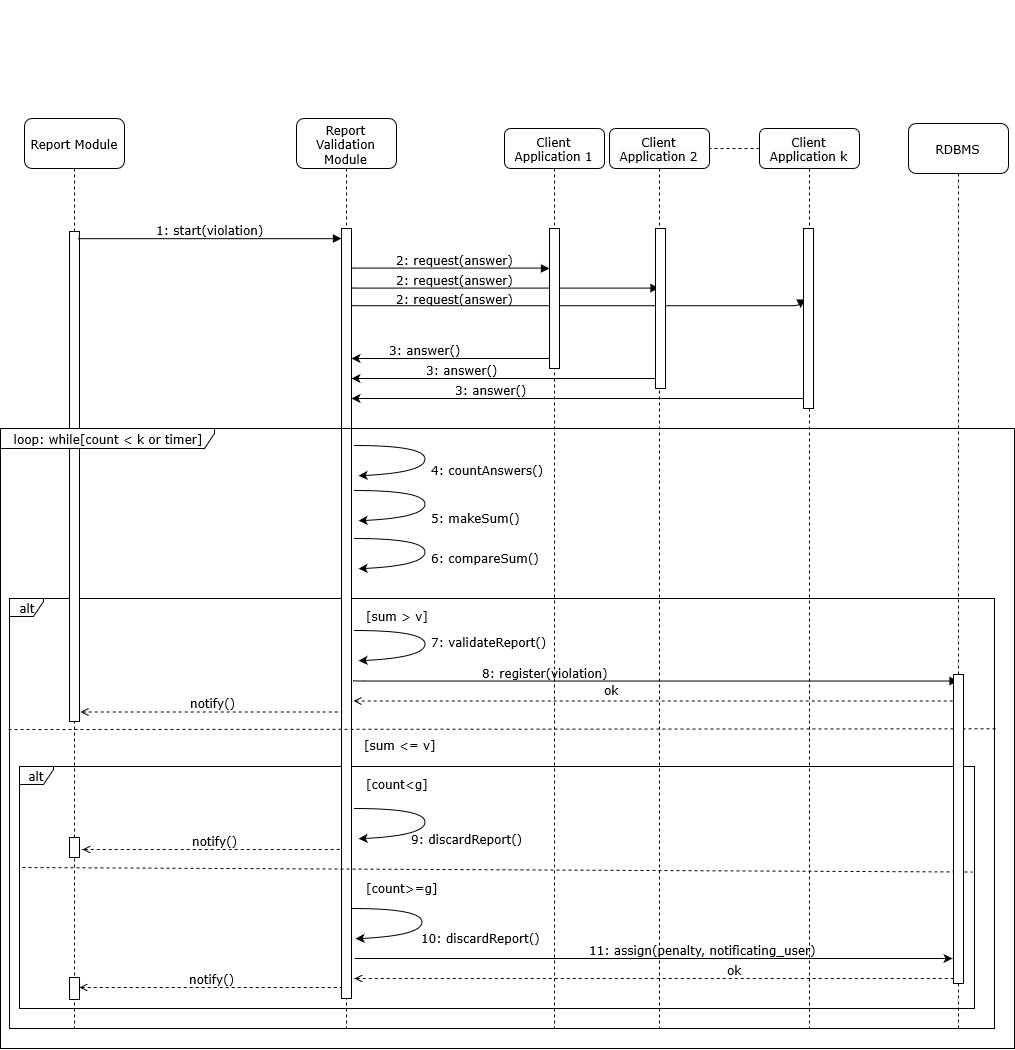
\includegraphics[width=\textwidth]{DD_Images/RunTimeView/3.jpg}
  \caption{\textit{Sequence diagram 3 - Validation of report}}
\end{figure}

\subsection{Statistic Display}
The diagram shows the workflow of the application during the visualization of statistics. The main component is the \textbf{StatisticsModule},
which contains the logic to access statistics data. The module contains the logic to show the user statistics when required by the Client Application
by inserting location of the desired area.

\begin{figure}[H]
  \centering
  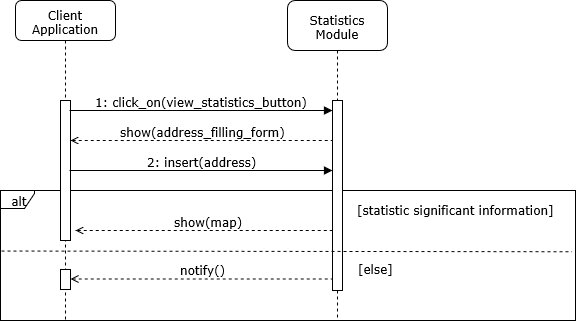
\includegraphics[width=\textwidth]{DD_Images/RunTimeView/4.jpg}
  \caption{\textit{Sequence diagram 4 - Statistics Display}}
\end{figure}

\subsection{Display to Authority Module of details of violations}
The diagram shows the workflow of the application during the display of data to AuthorityModule. The main components are the 
\textbf{LicensePlateModule} and the \textbf{AuthorityModule}. Once a license plate has been validated, the LicensePlateModule updates the 
number of violations connected to that license plate in the RDBMS. After this update, the AuthorityModule is called, to notify the validated 
license plate, and, as a consequence, it queries the RDBMS asking for history of the validated license plate. After the query, the AuthorityModule 
generates the traffic ticket.

\begin{figure}[H]
  \centering
  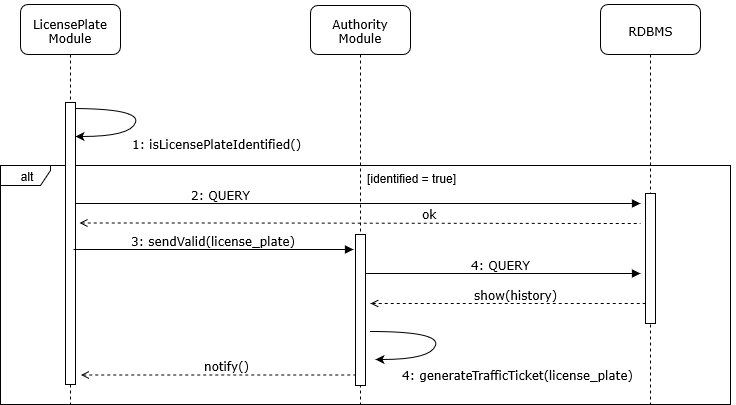
\includegraphics[width=\textwidth]{DD_Images/RunTimeView/5.jpg}
  \caption{\textit{Sequence diagram 5 - Display to Authority Module of details of violations}}
\end{figure}

\subsection{Update Profile to Authority}
The diagram shows the workflow of the application during the update of profile to authority. The main component is the \textbf{UserModule} 
that collects the data sent by the Client Application who asked for profile update, and interact with the Municipality to check data 
authenticity. When data are confirmed by the Municipality, the UserModule updates data on RDBMS regarding the Client Application who asked for 
profile update.

\begin{figure}[H]
  \centering
  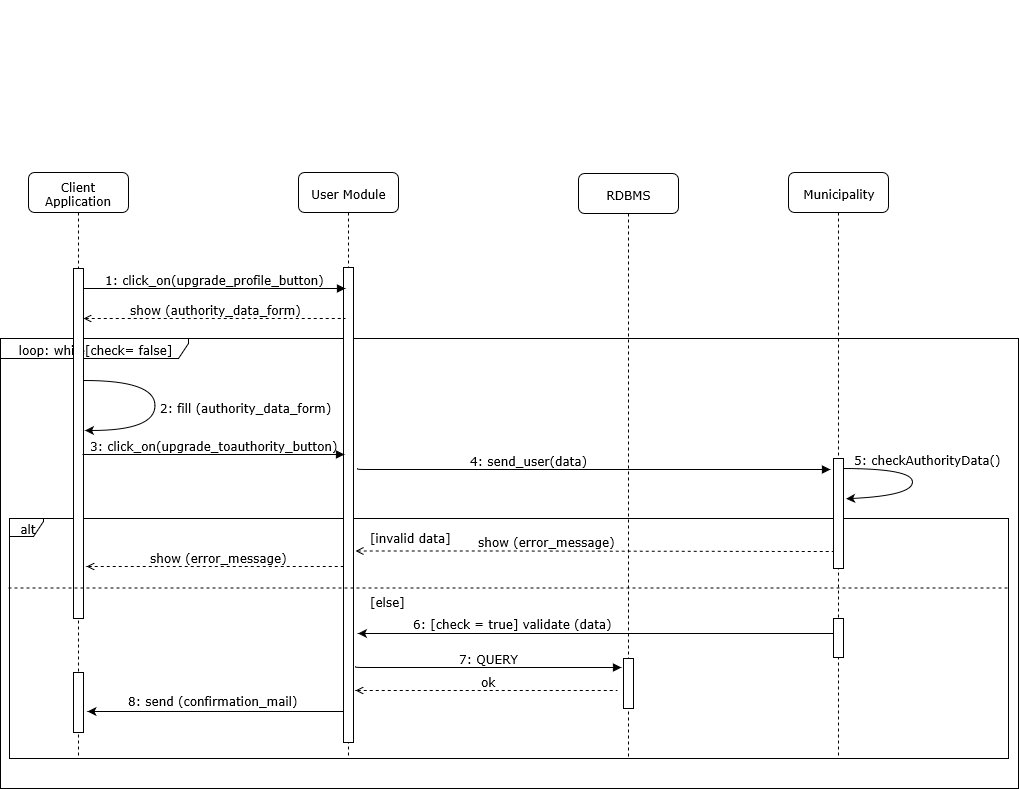
\includegraphics[width=\textwidth]{DD_Images/RunTimeView/6.jpg}
  \caption{\textit{Sequence diagram 6 - Update Profile to Authority}}
\end{figure}

\subsection{Update Statistics}
The diagram shows the workflow of the application during the update of statistics. The main component is the \textbf{StatisticsModule}, that
contains the logic to update statistics, collecting information by the Cloud Storage, at the first step, where information about pictures of 
violations are memorized. Then the module interacts also with the Municipality to increase the information collected by SafeStreets. In particular, 
the Municipality can provide more detailed information about car accidents, and other type of violations like this.

\begin{figure}[H]
  \centering
  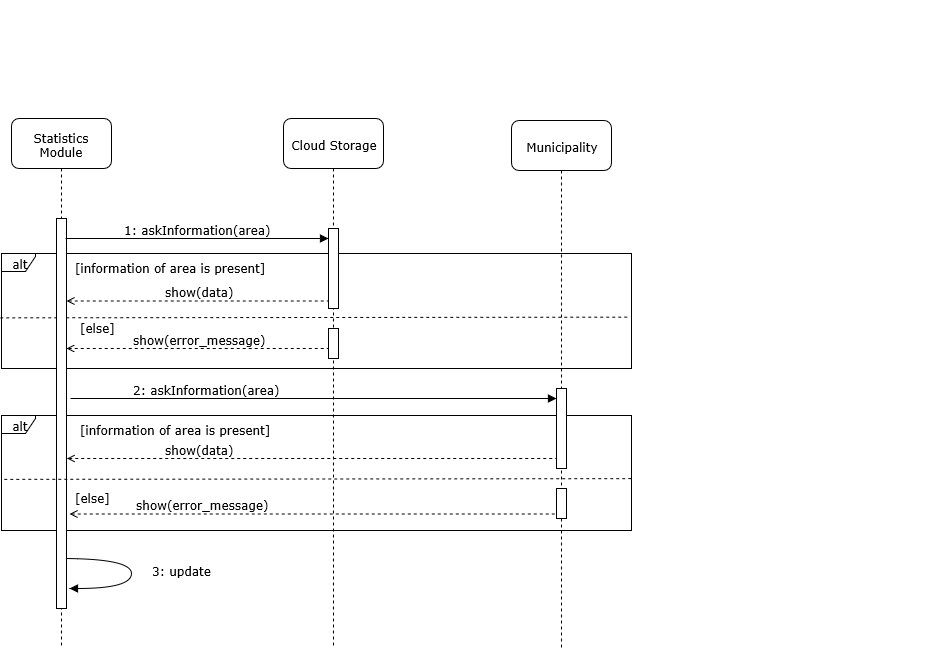
\includegraphics[width=\textwidth]{DD_Images/RunTimeView/7.jpg}
  \caption{\textit{Sequence diagram 7 - Update Statistics}}
\end{figure}

\subsection{Traffic Ticket Generation}
The diagram shows the workflow of the application during the generation of the traffic ticket. The main components are the 
\textbf{LicensePlateModule} and the \textbf{AuthorityModule}. Once a license plate has been validated, the LicensePlateModule queries the 
RDBMS to create a specific record for the new data. Subsequently, the AuthorityModule queries the RDBMS to have the license plate, and checks
if some information is missing. The module contains the logic to check integrity and completeness of data and to insert information, in case data 
are not complete. After the query, the AuthorityModule generates the traffic ticket.

\begin{figure}[H]
  \centering
  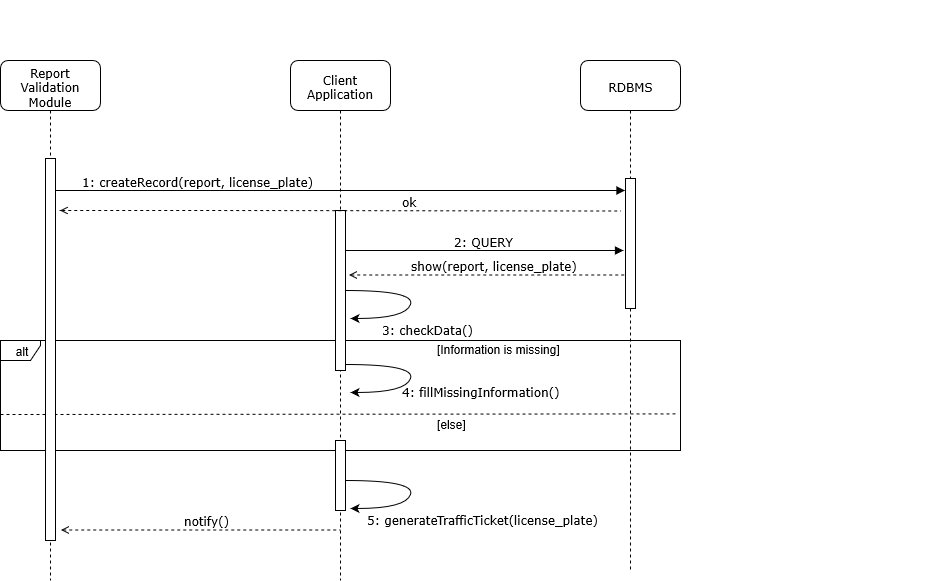
\includegraphics[width=\textwidth]{DD_Images/RunTimeView/8.jpg}
  \caption{\textit{Sequence diagram 8 - Traffic Ticket Generation}}
\end{figure}

